\section{Results}
\label{sec:results}

We now use the two routes together to answer the central question. The feature-space route asks what frozen SAM reveals before any proposal reasoning. The proposal-/mask-space route asks what can already be recovered from the generated mask bank under matched benchmark protocols. Read together, they separate latent organization in the representation from recoverable organization in the generated masks.

\subsection{What does the feature-space route reveal?}

Feature-space exploration gives a cautious positive answer to \textbf{RQ1} and a direct answer to \textbf{RQ2}. Appendix~\ref{app:feature_provenance} shows that a clustering-only probe over pooled coarse \texttt{backbone\_fpn} features recovers plausible texture partitions, that coarse scale dominates finer native-grid controls, and that positional debiasing such as flip-averaging materially changes what is recovered. Read under its archived probe protocol rather than as a leaderboard comparison, the feature route shows that frozen features already organize texture-relevant structure.

This route is informative precisely because the readout is so light. No decoder is trained and no proposal reasoning is required. When pooled coarse features already separate repeated-pattern regions, transition cases, and shape-versus-texture examples, it becomes hard to argue that frozen SAM is entirely texture-blind. What the feature route does not settle by itself is how much of that latent structure has already been externalized into the generated masks under matched benchmark evaluation.

\subsection{What does the proposal-/mask-space route reveal?}

\begin{table*}[t]
\centering
\scriptsize
\setlength{\tabcolsep}{5pt}
\renewcommand{\arraystretch}{0.98}
\begin{tabularx}{\textwidth}{@{}p{0.16\textwidth}p{0.28\textwidth}Xcc@{}}
\toprule
Benchmark & Evaluator / subset & Method & mIoU & ARI \\
\midrule
RWTD & official invariant, full-256 & SAM2.1-small original rerun~\cite{ravi2024sam2} & 0.1615 & 0.2183 \\
RWTD & official invariant, full-256 & \sys{} final & 0.4611 & 0.6966 \\
RWTD & official invariant, common-253 & TextureSAM public checkpoint rerun~\cite{texturesamrepo2026} & 0.4684 & 0.6163 \\
RWTD & official invariant, common-253 & \sys{} final & 0.4645 & 0.7013 \\
\midrule
STLD & direct foreground, all-200 & SAM2.1-small original rerun~\cite{ravi2024sam2} & 0.3686 & 0.5269 \\
STLD & direct foreground, all-200 & \sys{} final & 0.6705 & 0.7249 \\
STLD & direct foreground, common-182 & TextureSAM public checkpoint rerun~\cite{texturesamrepo2026} & 0.5140 & 0.7526 \\
STLD & direct foreground, common-182 & \sys{} final & 0.7195 & 0.7791 \\
\bottomrule
\end{tabularx}
\caption{Main matched comparisons. Each block fixes the evaluator and subset convention before comparing methods. Supporting bridge and CAID routes are reported separately in the appendix so that the headline table remains protocol-matched.}
\label{tab:proposal_results}
\end{table*}


Proposal-/mask-space exploration answers the complementary question. On RWTD, the raw SAM2.1-small baseline is far below either texture-specialized adaptation or a lightweight readout above the frozen mask bank. Against the matched TextureSAM rerun on the shared RWTD subset, the proposal route reaches comparable overlap quality while improving partition coherence from 0.6163 to 0.7013 ARI. Because the official RWTD no-aggregation metric averages matched GT instances rather than simple per-image scores, we summarize uncertainty on the same overlap-instance view used by the paired analysis: the ARI gain is $+0.0995$ with a 95\% paired bootstrap interval of [$0.0721$, $0.1270$], while mIoU changes by $+0.0405$ [$0.0031$, $0.0764$]. The full official evaluator supports the same reading: the proposal route remains far above the raw SAM baseline at 0.4611 mIoU / 0.6966 ARI.

STLD shows the same route under cleaner synthetic geometry. On the matched shared subset, the proposal route improves from 0.5140 / 0.7526 to 0.7195 / 0.7791, and paired per-image bootstraps remain positive on average across both the matched subset and all-image view. The ARI gain is smaller than the RWTD gain, but it remains directionally consistent with the claim that generated masks contain recoverable texture structure. Together, RWTD and STLD show that substantial texture task value can be recovered from the frozen mask bank without retraining the backbone or proposal generator.

Appendix~\ref{app:implementation_details} shows that this result is not reducible to one lucky descriptor stack and also reports the practicality profile of the readout. The hybrid descriptor helps most on the harder fragmented RWTD regime, but the proposal-route claim survives across descriptor families, and the measured runtime remains modest for a lightweight layer above a fixed bank.

\subsection{What do the two routes reveal together?}

The two routes are parallel in question but different in what they expose. Feature-space exploration reveals latent organization in the frozen representation before any explicit mask reasoning. Proposal-/mask-space exploration reveals whether that organization has already been externalized into the generated masks strongly enough to recover a coherent texture partition. The first route is therefore most informative about existence and localization of texture-relevant structure; the second is most informative about recoverability under matched end-task evaluation.

\begin{figure*}[t]
    \centering
    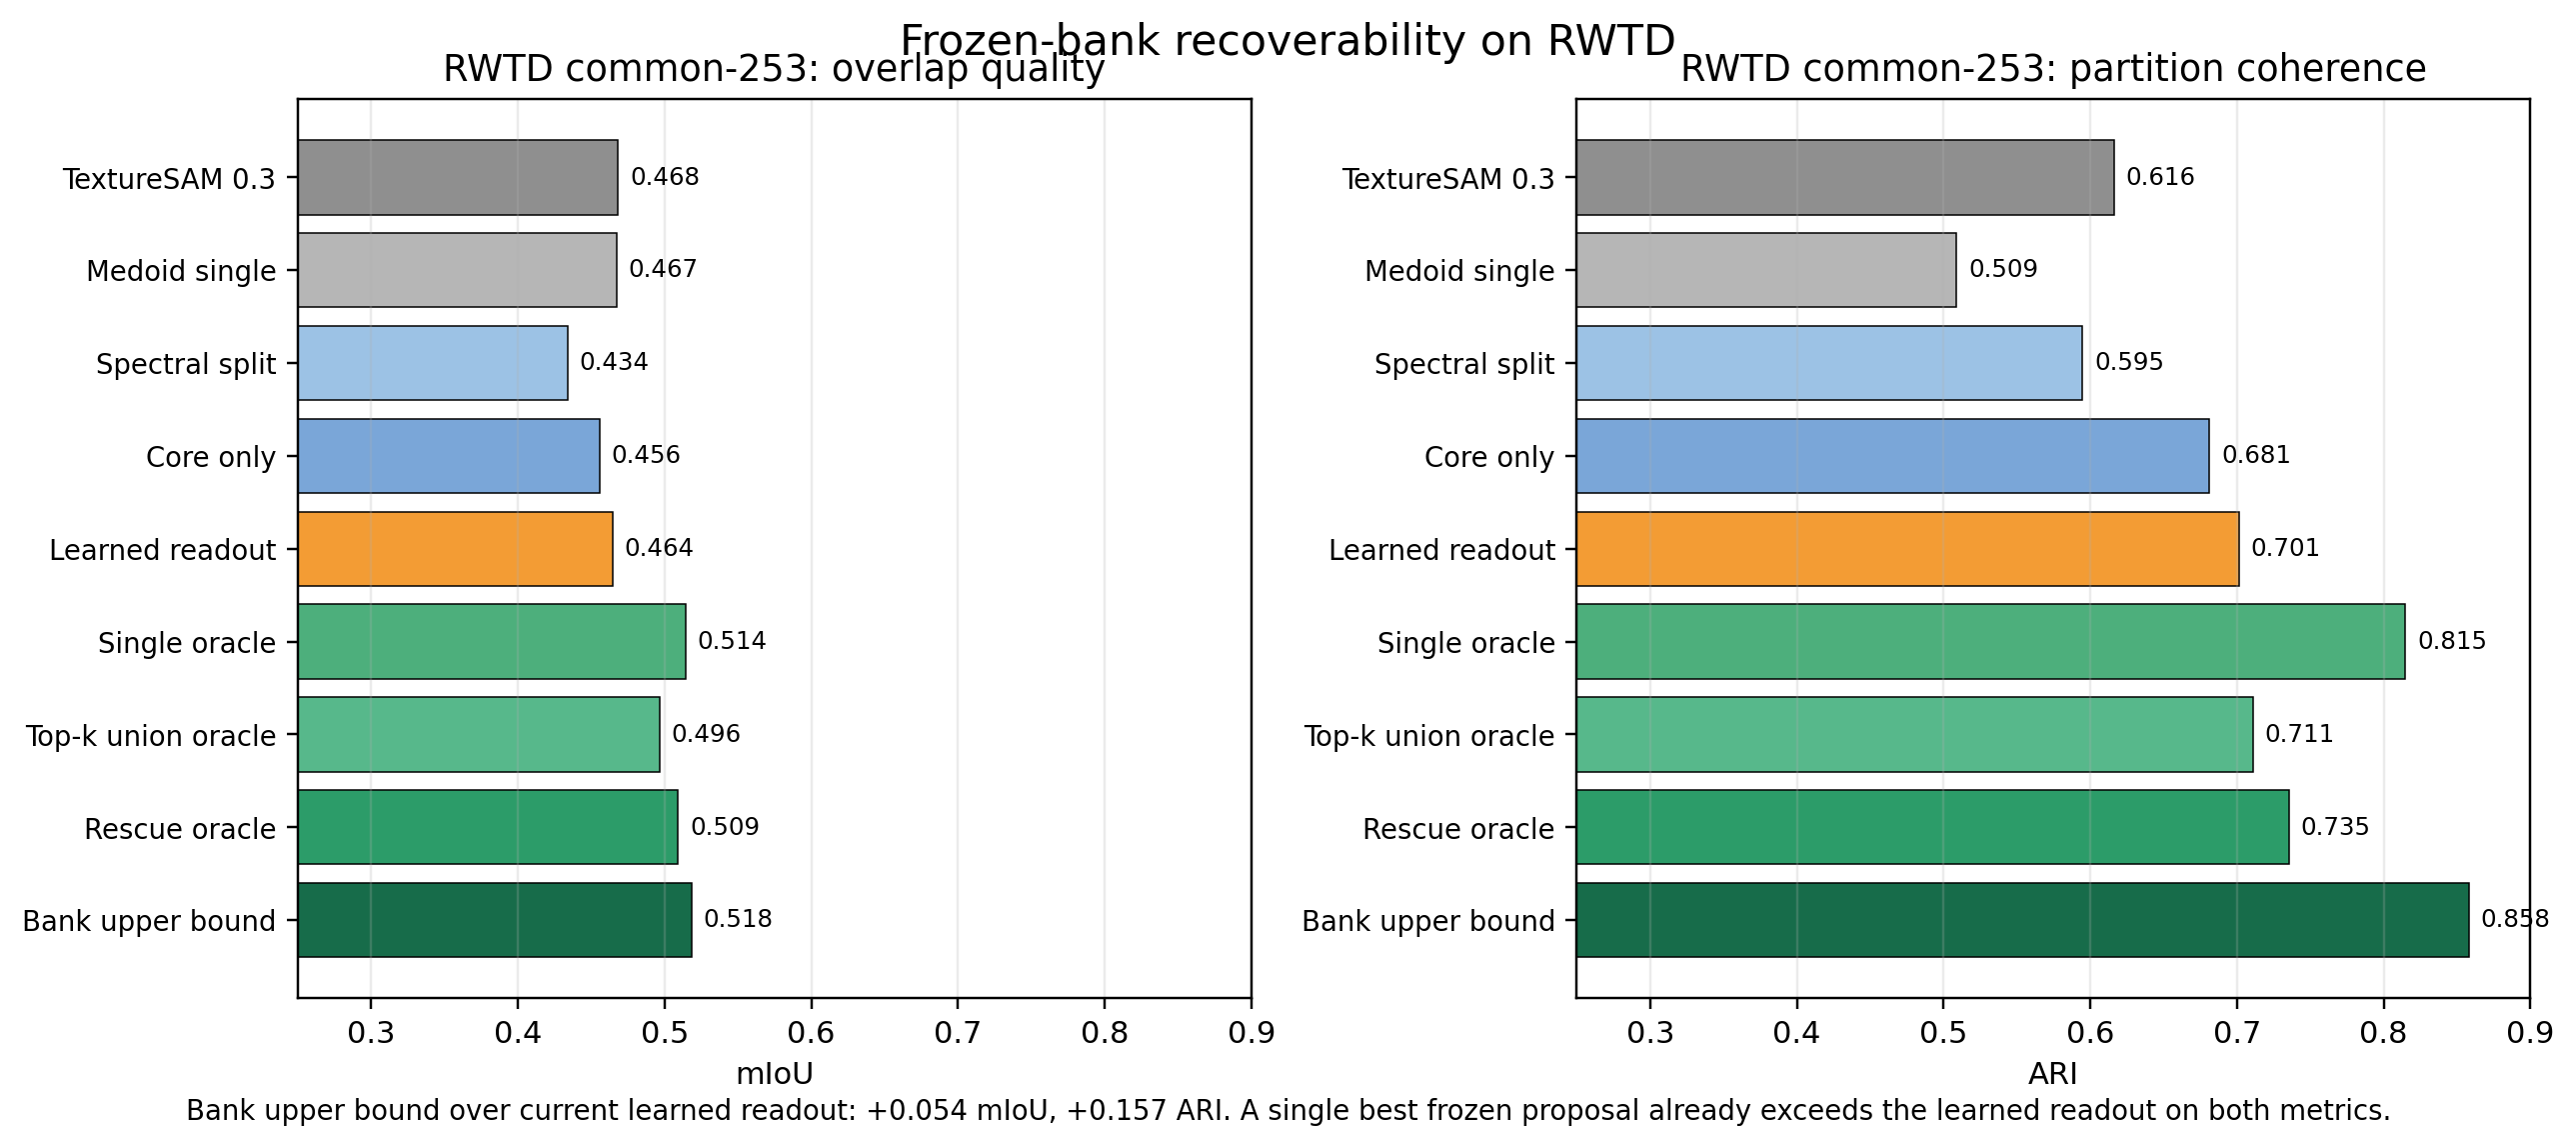
\includegraphics[width=0.98\textwidth]{figures/fig_rwtd_oracle_decomposition.png}
    \caption{Proposal-/mask-space route on RWTD. Generic frozen-bank heuristics are noticeably weaker than the learned readout, but the bank oracles remain substantially higher still. The figure therefore makes the route-specific message concrete: generated masks on natural fragmented scenes already contain substantial texture evidence, but that evidence is often distributed across fragments and low-margin alternatives.}
    \label{fig:rwtd_oracle_decomp}
\end{figure*}

\begin{table}[t]
\centering
\scriptsize
\begin{tabular}{@{}lcc@{}}
\toprule
RWTD common-253 method & mIoU & ARI \\
\midrule
Medoid single & 0.4673 & 0.5087 \\
Learned single selector & 0.4512 & 0.5601 \\
Spectral split & 0.4339 & 0.5948 \\
Agglomerative split & 0.4354 & 0.5898 \\
Greedy merge & 0.4442 & 0.5197 \\
Core only & 0.4558 & 0.6812 \\
\sys{} final & 0.4645 & 0.7013 \\
Single frozen-proposal oracle & 0.5142 & 0.8146 \\
Top-$k$ union oracle & 0.4964 & 0.7107 \\
Rescue candidate oracle & 0.5093 & 0.7352 \\
Bank upper bound & 0.5183 & 0.8580 \\
\bottomrule
\end{tabular}
\caption{RWTD recoverability decomposition on the matched common-253 subset. The learned top-1 selector is stronger than the medoid single baseline, but it still trails the full commitment stack by a wide ARI margin. The bank oracles remain far higher still. The omitted compatible-component oracle performs poorly (0.4748 mIoU / 0.2497 ARI), which is evidence that compatibility merging alone is not sufficient.}
\label{tab:oracle_recoverability}
\end{table}


RWTD makes \textbf{RQ4} concrete. A single frozen proposal can already be very strong, and the bank upper bound is higher still. Yet learned top-1 selection still trails the full readout by a wide ARI margin. The generated masks therefore contain substantial texture structure, but that structure is often distributed across multiple fragments or low-margin alternatives. This is where the proposal route reveals something the feature route cannot: the representation may already be organized, but the generated masks still need commitment to turn that organization into the right partition.

STLD gives the complementary answer. There, a learned single-proposal selector already nearly matches the full readout, which means the generated masks often already contain a coherent singleton answer. \Cref{tab:stld_selector_contrast} captures the regime contrast directly: RWTD is primarily a fragmented-evidence problem, while STLD is often a singleton-selection problem. Seen alongside the feature route, this contrast clarifies the joint interpretation. Frozen features expose texture organization broadly, while the generated masks determine whether that organization appears as fragmented evidence requiring commitment or as a nearly complete mask already available for selection.

\begin{table*}[t]
\centering
\scriptsize
\setlength{\tabcolsep}{5pt}
\renewcommand{\arraystretch}{0.98}
\begin{tabularx}{\textwidth}{@{}p{0.22\textwidth}Xcc@{}}
\toprule
Route & Variant & mIoU & ARI \\
\midrule
RWTD common-253 & Medoid single (generic bank baseline) & 0.4673 & 0.5087 \\
RWTD common-253 & Learned single selector & 0.4512 & 0.5601 \\
RWTD common-253 & Conservative core only & 0.4558 & 0.6812 \\
RWTD common-253 & Proposal route final & 0.4645 & 0.7013 \\
\midrule
STLD common-182 & Proposal union & 0.2543 & 0.1731 \\
STLD common-182 & Handcrafted consolidation & 0.3680 & 0.3987 \\
STLD common-182 & PTD heuristic & 0.3757 & 0.4085 \\
STLD common-182 & Learned single selector & 0.7196 & 0.7731 \\
STLD common-182 & Proposal route final & 0.7195 & 0.7791 \\
\midrule
ControlNet bridge all-1742 & Proposal union (synthetic complement) & 0.6749 & 0.1188 \\
ControlNet bridge all-1742 & Proposal route Stage-A (synthetic complement) & 0.6803 & 0.6039 \\
\bottomrule
\end{tabularx}
\caption{Route-specific evidence for \textbf{RQ4} using each route's native evaluator. On RWTD, learned top-1 selection helps but remains well below the structured commitment stack, while the conservative core already captures most of the coherence gain and the final rescue layer adds the remaining improvement. On STLD, by contrast, learned top-1 selection is already very strong, which highlights the difference between canonical synthetic partitions and the more fragmented natural RWTD scenes. The ControlNet bridge rows show that a simple proposal union remains inadequate even on the broader synthetic complement.}
\label{tab:proposal_ablation}
\end{table*}


Seen together, the routes suggest a simple joint interpretation. Frozen SAM is not missing texture structure altogether: the feature route reveals it internally, and the proposal route reveals that much of it has already been externalized into the generated mask bank. Their difference is where the unresolved difficulty lies. Features show that the representation is textured enough to support meaningful clustering; masks show that on natural fragmented scenes the remaining failure is commitment among partially correct proposals rather than total absence of relevant evidence.

\subsection{What remains unrecovered?}

The paper's answer is therefore incomplete in a precise way. Neither route fully closes ambiguity. The feature route can reveal latent organization, but it does not settle the final partition choice under matched benchmark evaluation. The proposal route can recover strong partitions, but the remaining oracle gap shows that the unresolved issue is less whether the mask bank ever contains the answer than whether the readout preserves multiple plausible hypotheses long enough to choose correctly. Appendix~\ref{app:rwtd_diag} expands this point with selector/core/final/oracle case studies, and Appendix~\ref{app:stld_support} shows the complementary STLD regime where a coherent singleton often already exists.
